\section{Umsetzung}


\begin{frame}
  \frametitle{Ansatz: Chunked-Swarm}
  Super-Peer teilt die Daten vor dem Transfer in kleine Teile (Chunks):
  \vspace{1mm}
  \begin{itemize}  
    \item Mindestens so viele Chunks wie Peers
    \item Peers beantragen disjunkte Chunks vom Super-Peer
    \item Peers tauschen Chunks untereinander aus
    \item Vereinfachung: Alle Peers haben die gleiche Uploadbandbreite
  \end{itemize} 
\end{frame}


\begin{frame}
  \frametitle{Chunked-Swarm: Ablauf}
  Beispiel: Genauso viele Chunks wie Peers
  \begin{exampleblock}{Phasen}  
    \begin{itemize}
      \item Phase 1 (links): Peers bekommen disjunkten Chunk vom Super-Peer
      \item Phase 2 (rechts): Peers tauschen ihre Chunks untereinander 
    \end{itemize}
  \end{exampleblock}
  \begin{center}
    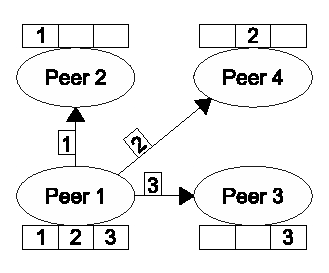
\includegraphics[width=0.4\textwidth]{fig/chunkedswarmmodel1.eps}
    \hspace{0.15\textwidth}
    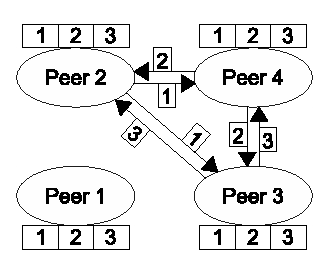
\includegraphics[width=0.4\textwidth]{fig/chunkedswarmmodel2.eps}
  \end{center}
\end{frame}


\begin{frame}
  \frametitle{Chunked-Swarm: Gesamtdauer}
  Beispiel: Genauso viele Chunks wie Peers
  \begin{exampleblock}{Zeitlicher Ablauf}
    \begin{itemize}
      \item Bis $T_0$: Super-Peer 1 schickt disjunkten Chunk an jeden Peer
      \item Ab $T_0$: Jeder Peer schickt Chunk an die anderen beiden Peers
      \item Ab $T_0 + \frac{2}{3} * T_0$: Daten wurden vollständig verbreitet
    \end{itemize}
  \end{exampleblock}
  \begin{center}
    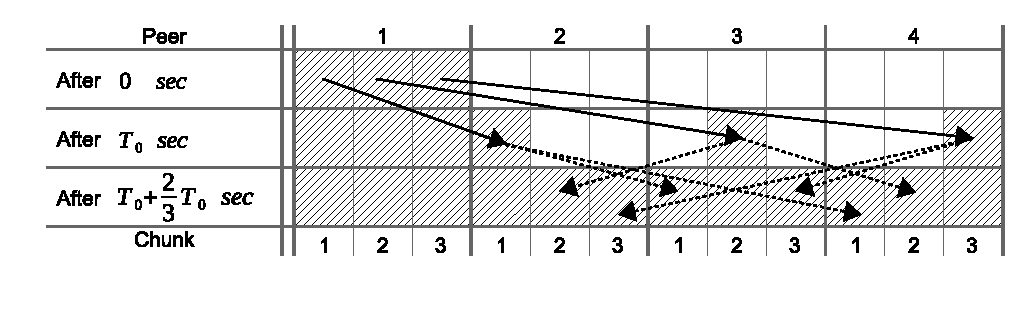
\includegraphics[width=1\textwidth]{fig/chunkedswarmformula1.eps}
  \end{center}
\end{frame}


\begin{frame}
  \frametitle{Chunked-Swarm: Gesamtdauer}
  \begin{block}{Eigenschaften}
    \begin{itemize}  
      \item Verdoppelung der Chunks halbiert die Zeit zwischen $T_0$ und Ende
      \vspace{2mm}
      \item Gesamtdauer: $T(n, c) = T_0\:+\:\frac{n}{c}\:*\:\frac{n-1}{n}\:*\:T_0$, $n \in \mathbb{N}_1$, $c = n\:*\:2^i, i \in \mathbb{N}_0$
      \vspace{2mm}
      \item Real-time: Gesamtdauer immer unter $2 * T_0$
    \end{itemize}
  \end{block}
\end{frame}


\begin{frame}
  \frametitle{Implementierung}
  \begin{itemize}  
    \item Mesh Topologie: Alle Peers sind miteinander verbunden
    \item Pull-Based: Chunks werden nur auf Wunsch übertragen
    \item Announcements: Jeder Peer kündigt seine Chunks an
    \item Automatic (Re-)Connect: Peers finden andere Peers durch Super-Peer
  \end{itemize} 
\end{frame}


\begin{frame}
  \frametitle{Implementierung}
  \begin{itemize}  
    \item Dead Peer Detection: Super-Peer verschickt Chunks erneut
    \item Traffic-Shaping: Up-/Downloadbandbreite drosselbar
    \item Implementiert in Java mit Netty5
  \end{itemize} 
\end{frame}


